\documentclass{beamer}

\usetheme{AAUsimple}

\usepackage{amsmath,amssymb,graphicx}
\usepackage{tikz}
\usetikzlibrary{arrows,decorations,decorations.markings}
\usepackage{listings}
\usepackage{upquote}
\newcounter{ipythoncounter}
\setcounter{ipythoncounter}{1}
\renewcommand{\ttdefault}{pcr}
\lstset{
  aboveskip=\bigskipamount,
  belowskip=\bigskipamount,
  basicstyle=\footnotesize\ttfamily,
  language=Python,
  numbers=left,
  stepnumber=9999,
  numberfirstline=true,
  xleftmargin=2cm,
}

\lstnewenvironment{ipythoninput} {
  \setcounter{lstnumber}{\value{ipythoncounter}} \renewcommand{\thelstnumber}
             {\bf\ttfamily In [\the\value{ipythoncounter}]:} \lstset{
               frame=single, frameround=tttt, name=ipythoninput, } } {
  \addtocounter{ipythoncounter}{1} }

\lstnewenvironment{ipythonoutput} { \addtocounter{ipythoncounter}{-1}
  \setcounter{lstnumber}{\value{ipythoncounter}} \renewcommand{\thelstnumber}
             {\bf\ttfamily Out[\the\value{ipythoncounter}]:} \lstset{
               name=ipythoninput } } { \addtocounter{ipythoncounter}{1} }

%% \newtheorem{theorem}{Theorem}
%% \newtheorem{definition}[theorem]{Definition}
%% \theoremstyle{definition}
%% \newtheorem{example}[theorem]{Example}

\DeclareMathOperator{\ZZ}{\mathbb{Z}}
\DeclareMathOperator{\RR}{\mathbb{R}}
\DeclareMathOperator{\CC}{\mathbb{C}}
\DeclareMathOperator{\hg}{\mathfrak{h}_g}
%% \DeclareMathOperator{\dx}{dx}
%% \DeclareMathOperator{\dt}{dt}
\newcommand{\dx}{\,\mathrm{d}x}
\newcommand{\dt}{\,\mathrm{d}t}
\newcommand{\dQ}{\,\mathrm{d}Q}
\DeclareMathOperator{\DivC}{\mathcal{C}}
\DeclareMathOperator{\DivD}{\mathcal{D}}
\DeclareMathOperator{\RCV}{\boldsymbol{K}}
\DeclareMathOperator{\Abel}{\boldsymbol{A}}
\DeclareMathOperator{\HalfLattice}{\Lambda_{1/2}}

\newcommand{\thchar}[2] {\begin{bmatrix}#1\\#2\end{bmatrix}}
\newcommand{\thcharsm}[2] {\left[ \begin{smallmatrix} #1
      \\ #2 \end{smallmatrix} \right]}



%%%%%%%%%%%%%%%%%%%%%%%%%%%%%%%%%%%%%%%%%%%%%%%%%%%%%%%%%%%%%%%%%%%%%%%%%%%%%%%
\title{Computing the Riemann Constant Vector}

\author{
  Chris Swierczewski\\
  {\tt cswiercz@uw.edu}
}

\date{21 April 2015}

\institute{
  Department of Applied Mathematics\\
  University of Washington\\
  Seattle, Washington
}

\pgfdeclareimage[height=1.5cm]{titlepagelogo}{AAUgraphics/aau_logo_new_circle}
\titlegraphic{
  \pgfuseimage{titlepagelogo}
}
%%%%%%%%%%%%%%%%%%%%%%%%%%%%%%%%%%%%%%%%%%%%%%%%%%%%%%%%%%%%%%%%%%%%%%%%%%%%%%%



%%%%%%%%%%%%%%%%%%%%%%%%%%%%%%%%%%%%%%%%%%%%%%%%%%%%%%%%%%%%%%%%%%%%%%%%%%%%%%%
\begin{document}
%%%%%%%%%%%%%%%%%%%%%%%%%%%%%%%%%%%%%%%%%%%%%%%%%%%%%%%%%%%%%%%%%%%%%%%%%%%%%%%

\begin{frame}[plain,noframenumbering]
  \titlepage
\end{frame}

%% \frame{
%%   \frametitle{Kadomtsev--Petviashvili Equation}
%%   $u(x,y,t) = $ surface height of a 2D periodic shallow water wave.
%%   \[
%%   \tfrac{3}{4} u_{yy} = \frac{\partial}{\partial x} \left(
%%   u_t - \tfrac{1}{4} \left(6uu_x + u_{xxx}\right) \right)
%%   \]

%%   \begin{columns}[T]
%%     \begin{column}{0.5\textwidth}
%%       \begin{figure}
%%         \centering
%%         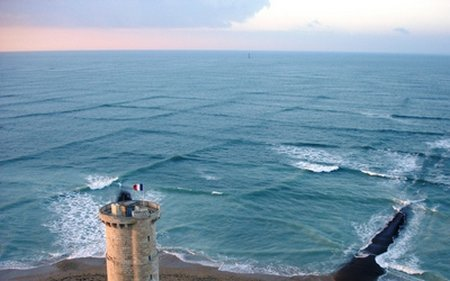
\includegraphics[width=\textwidth]{images/livekp.jpg}
%%         \caption{\^{I}le de R\'{e}, France}
%%       \end{figure}
%%     \end{column}
%%     \begin{column}{0.5\textwidth}
%%       \begin{figure}
%%         \centering
%%         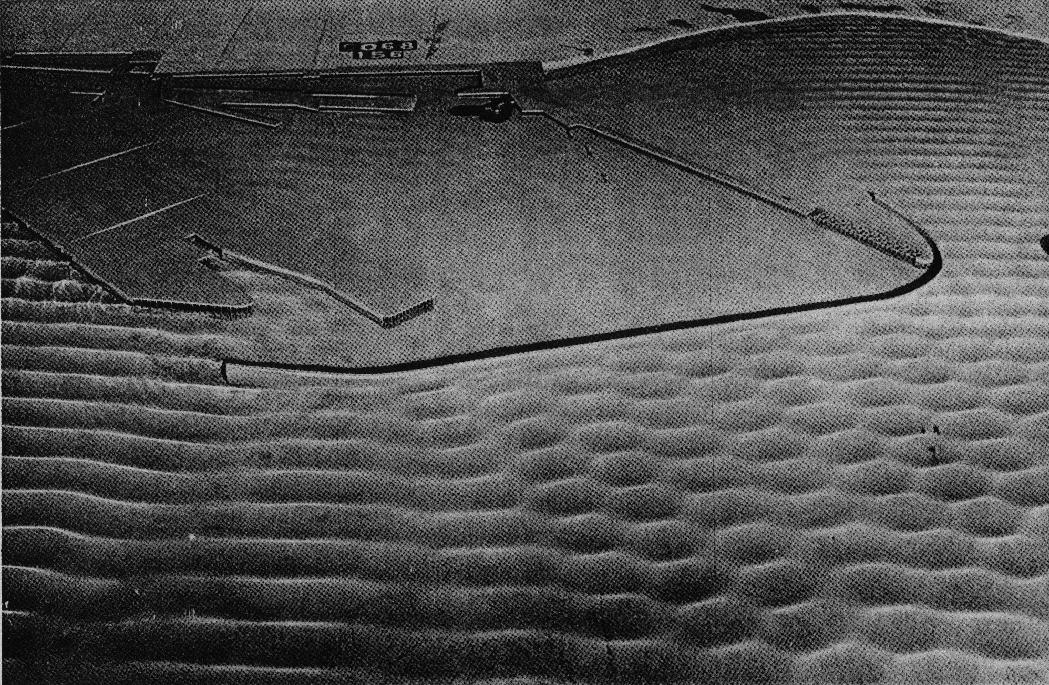
\includegraphics[width=\textwidth]{images/sd-harbor-model.jpg}
%%         \caption{Model of San Diego Bay}
%%       \end{figure}
%%     \end{column}
%%   \end{columns}

%% }

%% \frame{
%%   \frametitle{Kadomtsev--Petviashvili Equation}
%%   ``Finite-genus solutions:''

%%   \vspace{12pt}

%%   \[
%%   u
%%   =
%%   c + 2 \partial_x^2 \log \theta\Big( \boldsymbol{U}x +
%%   \boldsymbol{V}y + \boldsymbol{W}t + \Abel\big(P^\infty,\DivD\big) -
%%   \RCV(P^\infty), \Omega \Big)
%%   \]

%%   \vspace{12pt}

%%   \pause

%%   Quantities come from compact, connected, Riemann surfaces.
%% }


%% \frame{
%%   \frametitle{Whirlwind Background - Curves}

%%   \[
%%   C = \{ (\alpha, \beta) \in \CC^2 \; : \; f(\alpha, \beta) = 0 \}
%%   \]

%%   \pause
%%   \vspace{12pt}

%%   $C$ as a {\it $y$-covering} of $\CC_x^*$:
%%   \begin{itemize}[<+->]
%%     \item What are all possible $y$-roots to $f(x,y)=0$?
%%       \[
%%           x \mapsto y(x) = (y_1(x), \ldots, y_d(x))
%%       \]
%%   \end{itemize}

%%   \pause

%%   \begin{block}{Question:}

%%     Is there some surface other than $\CC_x^*$ where $y(x)$ is single-valued?
%%   \end{block}
%% }


%% \begin{frame}
%%   \frametitle{Whirlwind Background - Riemann Surfaces}
%%   (Compact) Riemann Surfaces $X$:

%%   \begin{itemize}[<+->]
%%     \item connected, 1-dimensional complex manifold,
%%     \item homeomorphic to a doughnut with $g$ holes,
%%       \begin{itemize}
%%         \item $g$ = {\it genus}
%%       \end{itemize}
%%     \item surface on which $y(x)$ is single-valued,
%%       \begin{itemize}
%%         \item (branch cuts, etc.)
%%         \item (caveats: singular points and points at infinity)
%%         \item (optional board demo for undergraduates)
%%       \end{itemize}
%%   \end{itemize}
%% \end{frame}


%% \begin{frame}{Whirlwind Background - Homology}
%%   \begin{figure}
%%   \centering
%%   \begin{tikzpicture}[scale=0.9]
%%     \colorlet{darkgreen}{green!50!gray}
%%     \colorlet{lightgray}{white!80!black}
%%     \colorlet{darkblue}{blue!50!gray}

%%     %% % Bezier Control Points
%%     %% \filldraw [gray] (-6,0) circle (2pt)
%%     %%                  (-6,1.5) circle (2pt)
%%     %%                  (-5,2.5) circle (2pt)
%%     %%                  (-3.5,2.5) circle (2pt)
%%     %%                  (-2,2.5) circle (2pt)
%%     %%                  (-1,1.5) circle (2pt)
%%     %%                  (0,1.5) circle (2pt);


%%     % the reference volume
%%     %\draw[lightgray, thick]         (0,-1.5) arc (270:90:0.4cm and 1.5cm);
%%     %\draw[lightgray, thick, dashed] (0,1.5)  arc (90:-90:0.4cm and 1.5cm);

%%     \begin{scope}[very thick]
%%     % Quadrant II of Torus
%%     % (other draw statements are flips / rotations)
%%     \draw (-6,0) ..
%%           controls (-6,1.5) and (-5,2.5) ..
%%           (-3.5,2.5) ..
%%           controls (-2,2.5) and (-1,1.5) ..
%%           (0,1.5);
%%     \draw[xscale=-1] (-6,0) ..
%%           controls (-6,1.5) and (-5,2.5) ..
%%           (-3.5,2.5) ..
%%           controls (-2,2.5) and (-1,1.5) ..
%%           (0,1.5);
%%     \draw[rotate=180] (-6,0) ..
%%           controls (-6,1.5) and (-5,2.5) ..
%%           (-3.5,2.5) ..
%%           controls (-2,2.5) and (-1,1.5) ..
%%           (0,1.5);
%%     \draw[yscale=-1] (-6,0) ..
%%           controls (-6,1.5) and (-5,2.5) ..
%%           (-3.5,2.5) ..
%%           controls (-2,2.5) and (-1,1.5) ..
%%           (0,1.5);

%%     % The Holes
%%     % (one hole at center shifted to outsides)
%%     \draw[xshift=-3.2cm] (-0.8,0) ..
%%           controls (-0.5,0.5) and (0.5,0.5) ..
%%           (0.8,0);
%%     \draw[yscale=-1,xshift=-3.2cm] (-1,-0.2) ..
%%           controls (-0.5,0.5) and (0.5,0.5) ..
%%           (1,-0.2);

%%     \draw[xshift=3.2cm] (-0.8,0) ..
%%           controls (-0.5,0.5) and (0.5,0.5) ..
%%           (0.8,0);
%%     \draw[yscale=-1,xshift=3.2cm] (-1,-0.2) ..
%%           controls (-0.5,0.5) and (0.5,0.5) ..
%%           (1,-0.2);

%%     \pause

%%     % a-cycles
%%     \draw[xshift=-3.2cm, darkblue, decoration={markings,
%%               mark=at position 0.25 with {\arrow[very thick]{latex}}},
%%           postaction={decorate}]
%%          (0,0) ellipse (2cm and 1.3cm);
%%     \draw[xshift=3.2cm, darkblue, decoration={markings,
%%               mark=at position 0.25 with {\arrow[very thick]{latex}}},
%%           postaction={decorate}]
%%          (0,0) ellipse (2cm and 1.3cm);

%%     % b-cycles
%%     \draw[xshift=-3.2cm, yshift=-2.47cm,
%%           darkgreen, decoration={markings,
%%               mark=at position 0.25 with {\arrow[very thick]{latex}}},
%%           postaction={decorate}]
%%          (0,0) arc (270:90:0.4cm and 1.07cm);
%%     \draw[xshift=-3.2cm, yshift=-0.33cm, dashed, darkgreen]
%%          (0,0) arc (90:-90:0.4cm and 1.07cm);
%%     \draw[xshift=3.2cm, yshift=-2.47cm,
%%           darkgreen, decoration={markings,
%%               mark=at position 0.25 with {\arrow[very thick]{latex}}},
%%           postaction={decorate}]
%%          (0,0) arc (270:90:0.4cm and 1.07cm);
%%     \draw[xshift=3.2cm, yshift=-0.33cm, dashed, darkgreen]
%%          (0,0) arc (90:-90:0.4cm and 1.07cm);

%%     % cycle labels
%%     \draw (-4,1.7)  node {$a_1$};
%%     \draw (4,1.7)   node {$a_2$};
%%     \draw (-3.2,-3) node {$b_1$};
%%     \draw (3.2,-3)  node {$b_2$};


%%     % cycle intersection properties
%%     \draw (0,-2.5)   node {$a_i \circ a_j = 0$};
%%     \draw (0,-3) node {$b_i \circ b_j = 0$};
%%     \draw (0.1,-3.5) node {$a_i \circ b_j = \delta_{ij}$};
%%     \draw (0,-4) node
%%     {$H_1(X,\mathbb{Z}) = \text{span}\{a_1,\ldots,a_g,b_1,\ldots,b_g\}$};

%%     \end{scope}
%%   \end{tikzpicture}
%%   \end{figure}
%% \end{frame}


%% \begin{frame}
%%   \vspace{32pt}
%%   \begin{center}
%%     {\Huge \it Demo}

%%     \vspace{24pt}

%%     Homology Basis
%%   \end{center}
%% \end{frame}


%% \begin{frame}{Whirlwind Background - One-Forms}{}
%%   {\bf Integration: natural use for paths.}

%%   {\it 1-forms}:
%%   \[
%%       \omega \in \Omega_X^1,
%%   \]
%%   where, it is {\it locally} written
%%   \[
%%       \omega \Big|_{U_\alpha \subset X} =
%%       h_\alpha\big(x,y(x)\big)dx, \quad h_\alpha \text{ meromorphic}.
%%   \]

%%   \uncover<2>{
%%   Given a path
%%   \[
%%       \gamma \in H_1(X,\mathbb{Z})
%%   \]
%%   we can compute
%%   \[
%%       \int_\gamma \omega.
%%   \]
%%   }
%% \end{frame}

%% %------------------------------------------------------------------------------
%% \section*{Abel Map}
%% %------------------------------------------------------------------------------

%% \begin{frame}{The Abel Map}{}

%%   Let $P \in X$ be a fixed place. The Abel Map
%%   \[
%%   \Abel : X \to J(X)
%%   \]

%%   \pause

%%   is defined by
%%   \[
%%   \Abel(P,Q) = \big( A_1(P,Q), \ldots, A_g(P,Q) \big),
%%   \]
%%   where
%%   \[
%%   A_j(P,Q) = \int_P^Q \omega_j.
%%   \]

%%   \pause

%%   \begin{block}{Abel Map on Divisors}
%%     If $\DivD = \sum_i n_i P_i$ then
%%     \[
%%     \Abel(P,\DivD) = \sum_i n_i \bold \Abel(P,P_i)
%%     \]
%%   \end{block}
%% \end{frame}


%% \begin{frame}
%%   \vspace{32pt}
%%   \begin{center}
%%     {\Huge \it Demo}

%%     \vspace{24pt}

%%     The Abel Map
%%   \end{center}
%% \end{frame}


%% \begin{frame}{Riemann Constant Vector}
%%   The Riemann constant vector
%%   \[
%%   \RCV : X \to J(X)
%%   \]

%%   \pause

%%   is defined as
%%   \[
%%   \RCV(P) = \big( K_1(P), \ldots, K_g(P) \big),
%%   \]
%%   where
%%   \[
%%   K_j(P) = \frac{1 + \Omega_{jj}}{2} - \sum_{k \neq j}^g
%%            \oint_{a_k} \omega_k(Q) A_j(P,Q) \dQ.
%%   \]
%% \end{frame}


\begin{frame}{Riemann Constant Vector}
  \[
  K_j(P) = \frac{1 + \Omega_{jj}}{2} - \sum_{k \neq j}^g
           \oint_{a_k} \omega_k(Q) A_j(P,Q) \dQ
  \]

  \begin{itemize}
  \item Double integral: difficult to compute.
  \end{itemize}

  \pause

  \begin{block}{Theorem}
    Let $P_0,P \in X$. Then
    \[
    \RCV(P) = \RCV(P_0) + (g-1)\Abel(P_0,P).
    \]
  \end{block}

  \pause

  \begin{itemize}
  \item Idea: most work to compute $\RCV(P_0)$ \underline{once}.
  \end{itemize}
\end{frame}

\begin{frame}{Computing the RCV}{}

  \vspace{12pt}

  Algorithm to compute $\RCV(P_0)$ inspired by two theorems:

  \vspace{24pt}

  \begin{block}{Theorem}
    \alt<1>{
      Let $\DivC$ be a divisor of degree $2g-2$. Then $\DivC$ is a
      canonical divisor if and only if
      \[
      2 \RCV(P) \equiv - \Abel(P,\DivC).
      \]
      \vspace{4in}
    }{
      A vector $\boldsymbol{W} \in J(X)$ satisfies
      \[
      \theta(\boldsymbol{W}, \Omega) = 0,
      \]
      if and only if $\exists \DivD = P_1 + \cdots + P_{g-1}$ such that
      \[
      \boldsymbol{W} = \Abel(P,\DivD) + \RCV(P).
      \]
      \vspace{4in}
    }
  \end{block}
  \visible<2->{}
\end{frame}


\begin{frame}{Computing the RCV}{}
  Combining the theorems:
  \begin{enumerate}[<+->]
  \item compute a canonical divisor $\DivC$,
  \item solve the equation
    \[
    2 \RCV(P_0) \equiv - \Abel(P_0,\DivC),
    \]
  \item validate using
    \[
    \theta\Big(\Abel(P_0,\DivD) + \RCV(P_0), \Omega \Big) = 0,
    \]
  \end{enumerate}
\end{frame}


\begin{frame}{1. Computing a Canonical Divisor}{}
  Meromorphic differential:
  \[
  \eta = \frac{p(x,y) \dx}{q(x,y)}
  \]

  \vspace{12pt}

  Valuation divisor:
  \[
  (\eta)_\text{val} = \sum_i p_i P_i - \sum_j q_j Q_j
  \]
  where $P_i, Q_i \in X$ are poles and zeros, resp.
\end{frame}


\begin{frame}{1. Computing a Canonical Divisor}{}
  Given $P \in X$, \\
  \[
  P = \big( x_P(t), y_P(t) \big),
  \]

  \vspace{12pt}
  a \underline{necessary} condition for $P \in (\eta)_\text{val}$ is \\

  \begin{gather*}
    p\big(x_P(t), y_P(t)\big) \Big|_{t=0} \! = 0,
    \qquad
    q\big(x_P(t), y_P(t)\big) \Big|_{t=0} \! = 0, \\
    \qquad \text{or} \quad
    \frac{\dx_P}{\dt}\big(0\big) = x_P'(t)dt \Big|_{t=0} = 0.
  \end{gather*}
\end{frame}


\begin{frame}
  \vspace{32pt}
  \begin{center}
    {\Huge \it Demo (Brief)}

    \vspace{24pt}

    Localizing Differentials at Places
  \end{center}
\end{frame}


\begin{frame}{1. Computing a Canonical Divisor}{}
  Use the Abelian differentials of the 1st kind:
  \[
  \omega_i = \frac{p_i(x,y) \dx}{\partial_y f(x,y)}
  \]
\end{frame}


%%%%%%%%%%%%%%%%%%%%%%%%%%%%%%%%%%%%%%%%%%%%%%%%%%%%%%%%%%%%%%%%%%%%%%%%%%%%%%%
\end{document}
%%%%%%%%%%%%%%%%%%%%%%%%%%%%%%%%%%%%%%%%%%%%%%%%%%%%%%%%%%%%%%%%%%%%%%%%%%%%%%%
